Let $f(\mathbf{x})$ be a function, where $\mathbf{x} \in \mathbb{R}^d$.
The \textit{level surface} of a function is the set of points with the same value of function, \ie
\begin{equation}
    L_c = \left\{ \mathbf{x} \mid f(\mathbf{x}) = c \right\} \label{q11.ls}
\end{equation}
for some c $\in$ $\mathbb{R}$. 

\begin{figure}[h!]
    \centering
    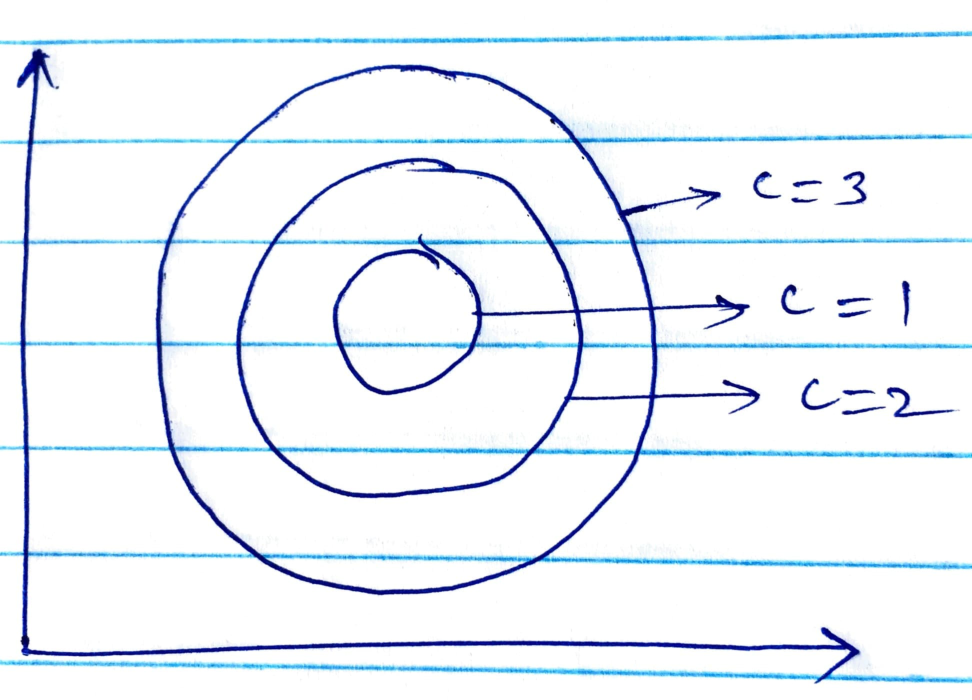
\includegraphics[scale=0.5]{circle_dl.pdf}
\end{figure}

The above figure shows level surfaces for different values of c for a 2-dimensional case. The points on the perimeter of each curve illustrate the set of points sharing the same value, i.e. $f(x_1, x_2) = c$.

Recall that a gradient vector is defined as $\nabla f = \left[ \frac{\partial f}{\partial x_1}, \frac{\partial f}{\partial x_2}, ..., \frac{\partial f}{\partial x_d} \right]$.

Consider a specific point $\mathbf{x}_0 \in \mathbb{R}^d$. Let us denote the level surface passing through this point by $L_{f(\mathbf{x_0})}$. Let us denote the gradient vector at $\mathbf{x_0}$ by $\nabla f_0$. 

Now, consider an arbitrary curve $\mathbf{r}(t) = \left[x_1(t); x_2(t); \ldots, x_d(t)\right]$ (parameterized by a scalar $t$) that passes through $\mathbf{x}_0$, 
\ie $\mathbf{r}(t_0) = \mathbf{x_0}$ for some $t_0 \in \mathbb{R}$. Furthermore, 
the curve $\mathbf{r}(t)$ lies within the level surface passing through $\mathbf{x}_0$, \ie $\mathbf{r}(t) \in L_{f(\mathbf{x_0})}, \,\, \forall t$.  

Recall that the \emph{tangent} to a curve is defined as $\frac{\del \mathbf{r}}{\del t}$. 

%lies within the level surface, \ie $\mathbf{r}(t) \in L$  where $\mathbf{r}(0) = \mathbf{x_0}$, i.e. it passes through $x_0$. 

With all that context and notation behind us, now comes the `fun' part -- 
show that $\nabla f_0$ is orthogonal to the tangent of $\mathbf{r}(t)$ at $t_0$. 

Now, please describe in non-technical language what you have just proven. Why might we care about this in the context of deep learning? 

